\section{Spørgsmål 6}

% Hvad er Relationel Algebra (RA)? Kom herunder ind på: relation, tuple, set og operatorer (select, projection, join...) samt RA' betydningen for opbygningen af  SQL (Structured Querry Language) erklæringer

\subsection{Fokuspunkter}
\begin{itemize}
	\item Hvad er Relationel Algebra (RA)?
	\begin{itemize}
		\item Kom herunder ind på: relation, tuple, set og operatorer (select, projection, join...).
	\end{itemize}
	\item Samt RA' betydningen for opbygningen af  SQL (Structured Querry Language) erklæringer.
\end{itemize}

\subsection{Litteratur}
\begin{itemize}
	
%	\item Fra teori: Database Modeling and Design. Logical Design 5'th Ed.
%	\begin{itemize}
%		\item Ch. 1 (p1 - 11)
%		\item Ch. 2 (p13 - 34)
%		\item Ch. 3 (p35 - 53)
%		\item Ch. 4 (p55 - 84)
%	\end{itemize}
	
	\item Fra Database eLearning: \url{http://db.grussell.org/index.html}.
	\begin{itemize}
		\item Ralational Algebra.
		\begin{itemize}
			\item \href{http://db.grussell.org/section010.html}{Introduction to Relational Algebra}.
			\item \href{http://db.grussell.org/section011.html}{Algebraic format Relational Algebra}.
		\end{itemize}
	\end{itemize}
	
%	\item Fra wikipedia:
%	\begin{itemize}
%		\item 
%	\end{itemize}
%	
%	\item Fra Agile Data Home Page:
%	\begin{itemize}
%		\item 
%	\end{itemize}
\end{itemize}

\newpage

% must
\subsection{Hvad er Relationel Algebra (RA)?}

%\textit{"There must be a set of rules which state how the database system will behave. For instance, somewhere in the DBMS\footnote{Database management system.} must be a set of statements which indicate, when someone inserts data into a relation, it has the effect which is expected. One way to specify this is to write an `essay' as to how the DBMS will operate, but words are imprecise and open to interpretation. Instead, relational databases are usually defined using Relational Algebra."}\\

Relationel algebra er \textbf{en entydig måde at beskrive en database's opførsel på}: 

\begin{itemize}
	\item The formal description of how a relational database operates.
	\item An interface to the data stored in the database itself.
	\item The mathematics which underpin SQL operations.
\end{itemize}

Videre så forklare teksten: \textit{"Operators in relational algebra are not the same as SQL operators, even if they have the same name. For example, the SELECT statement exists in SQL, and in RA. These two uses of SELECT are not the same. The DBMS takes whatever SQL statements the user types and translate them into RA operations before applying them to the database."}\\

Videoerne i nedstående playliste var \textbf{meget} brugbare:\\
\textit{Relational Algebra 1 - Select and Project Operators}:\\
\url{https://www.youtube.com/watch?v=yVh_LcOcQdg&list=PL8A52AA7E276200C0&index=1}

% must
\subsection{Kom herunder ind på: relation, tuple, set og operatorer (select, projection, join...)}

Fremragende beskrivelse af alle operatorer og alt andet kan også findes her: \\
\url{http://db.grussell.org/section010.html#_Toc67114476}


\subsubsection{Terminologi}

\begin{table}[H]
	\begin{tabu}{lX}
		\toprule
		\textbf{Navn} & \textbf{Beskrivelse}\\
		\midrule
		Relation & Et set af tupler\\
		Tuple & Er en samling af attributter\\
		Attribut & Er en kolonne\\
		Domæne & Er typen af data i en kolonne\\
		Set & Matematisk definition af en samling objekter i en relation, \textit{ingen} dubletter\\
		Udtryk & $operator_{betingelse}(\text{tabel})$\\
		\bottomrule
	\end{tabu}
	\caption{Beskrivelser af termer indenfor Relationel Algebra.}
\end{table}

Der er ikke 'nøgler' i RA. Nøgler er er teknisk implementering, for at opfylde regler indenfor RA.

%Et udtryk vil være på denne form:
%
%\begin{equation*}
%operator_{betingelse}(\text{i tabel})
%\end{equation*}

%Til beskrivelse af diverse operatorer bruger vi tabel \ref{tab:stud}.
%
%\begin{table}[H]
%	\centering
%	\begin{tabular}{lrrl}
%		\toprule
%		\textbf{Navn}	&\textbf{Alder}	&\textbf{Gennemsnit}&\textbf{Email}\\
%		\midrule
%		John Derp		& 24 			& 7,7	& john@derp.me			\\			
%		Hans Hansen		& 45 			& 9,8	& hans@landmand.dk		\\			
%		Brian Jensen	& 22 			& 4,5	& brian@randers.dk		\\			
%		Signe Andersen	& 25 			& 8,6	& signe@hotmail.com		\\
%		\bottomrule
%	\end{tabular}
%	\caption{Tabel over studerende.}
%	\label{tab:stud}
%\end{table}
\subsubsection{Set operationer}

Er operationer vi kan lave på tværs af forskellige Set, semantik er beskrevet ved hjælp af figur~\ref{fig:union_intersection_difference}. Eksempler på brug af disse kan ses på figur~\ref{fig:union_intersection_difference_example}

\begin{figure}[H]
	\centering
	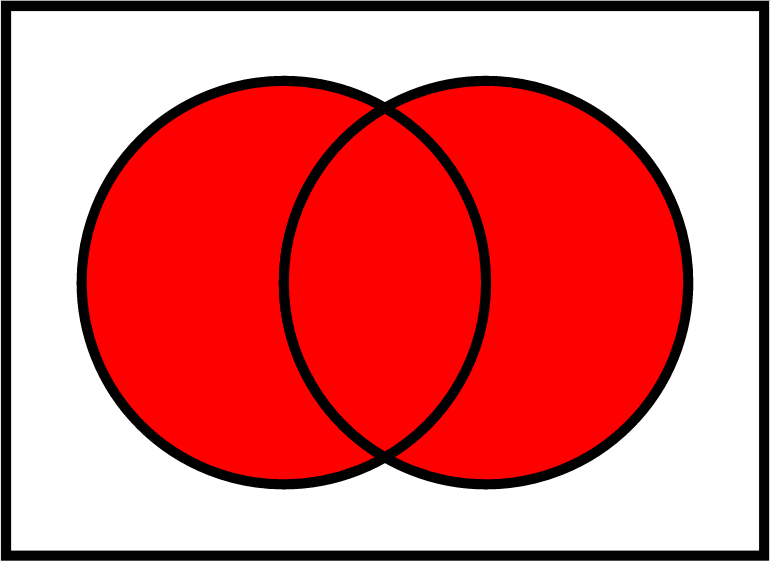
\includegraphics[width=.3\textwidth]{figs/spm6/union}\hfill
	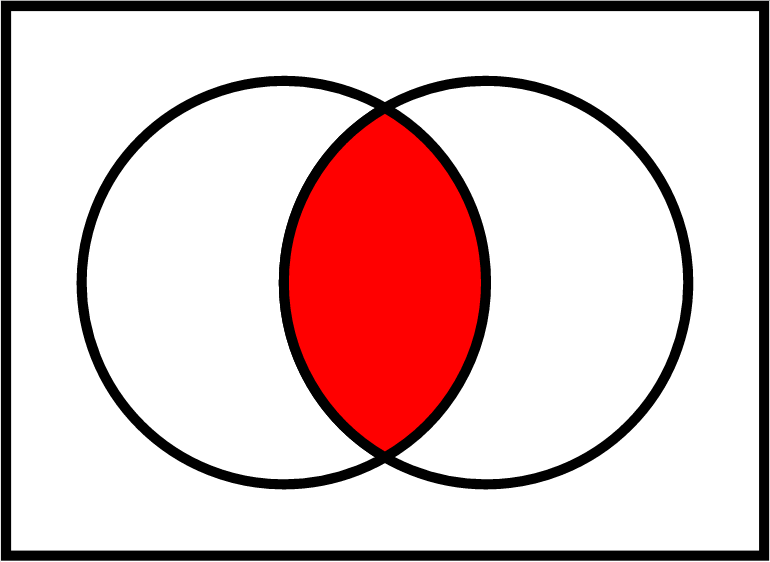
\includegraphics[width=.3\textwidth]{figs/spm6/intersection}\hfill
	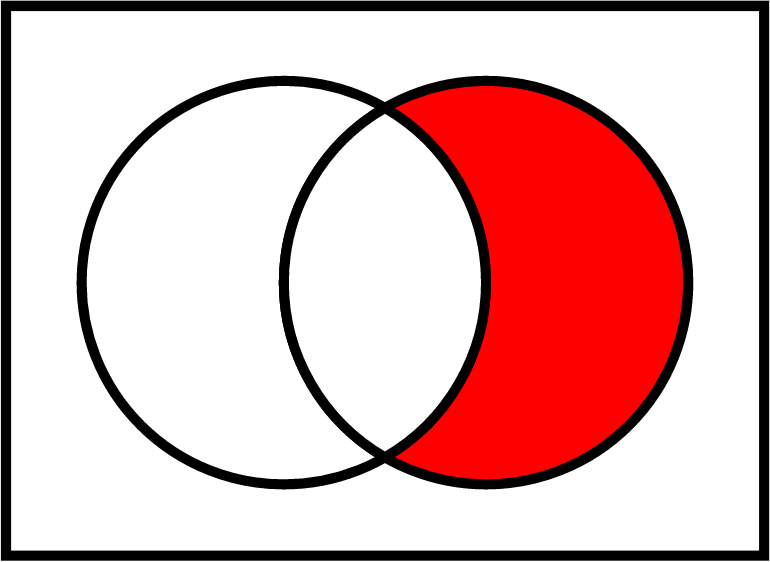
\includegraphics[width=.3\textwidth]{figs/spm6/difference}
	
	\caption{\href{https://en.wikipedia.org/wiki/Union_(set_theory)}{UNION} (tv), \href{https://en.wikipedia.org/wiki/Intersection_(set_theory)}{INTERSECTION} (midt) og \href{https://en.wikipedia.org/wiki/Complement_(set_theory)}{DIFFERNENCE} (tv).}
	\label{fig:union_intersection_difference}	
\end{figure}

Hvis vi har to relationer R og S (taget fra \href{http://db.grussell.org/section010.html#_Toc67114476}{udleveret materiale}). 

\begin{itemize}
	
	\item \textbf{UNION of R and S:}\\
	The union of two relations is a relation that includes all the tuples that are either in R or in S or in both R and S. Duplicate tuples are eliminated.
	
	\item \textbf{INTERSECTION of R and S:}\\
	The intersection of R and S is a relation that includes all tuples that are both in R and S.
	
	\item \textbf{DIFFERENCE of R and S:}\\
	The difference of R and S is the relation that contains all the tuples that are in R but that are not in S.
\end{itemize}

\begin{figure}[H]
	\centering
	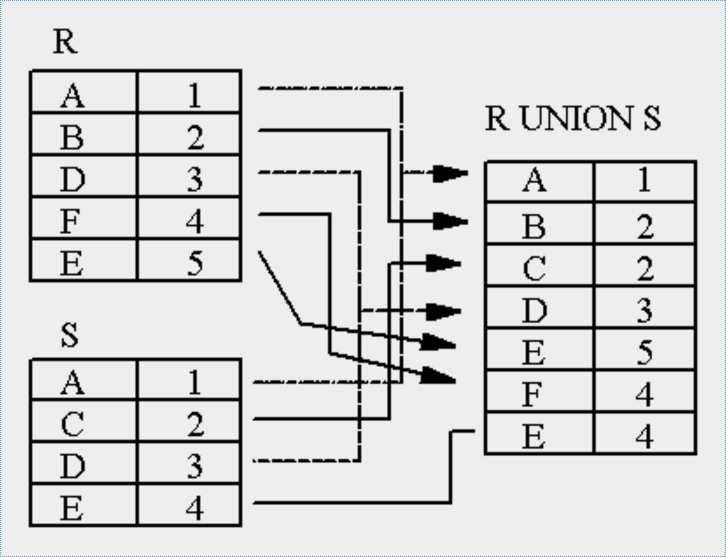
\includegraphics[width=.33\textwidth]{figs/spm6/unionexample}\hfill
	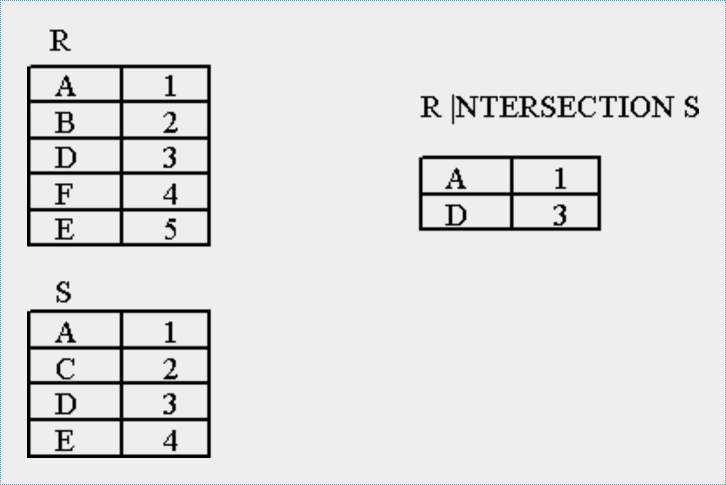
\includegraphics[width=.33\textwidth]{figs/spm6/intersectionexample}\hfill
	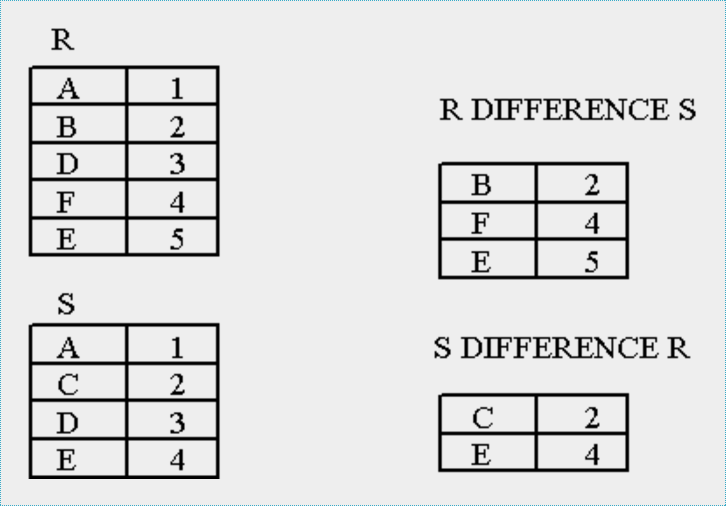
\includegraphics[width=.33\textwidth]{figs/spm6/differenceexample}
	
	\caption{\href{https://en.wikipedia.org/wiki/Union_(set_theory)}{UNION} (tv), \href{https://en.wikipedia.org/wiki/Intersection_(set_theory)}{INTERSECTION} (midt) og \href{https://en.wikipedia.org/wiki/Complement_(set_theory)}{DIFFERNENCE} (tv).}
	\label{fig:union_intersection_difference_example}	
\end{figure}

\paragraph{Krav}

For at kunne udføre disse operationer skal nogle betingelser være opfyldt: 

\begin{itemize}
	\item Relationerne (tabellerne) skal have samme antal kolonner.
	\item Domænerne skal være ens (kolonnerne skal indeholde de samme type data).
\end{itemize}
\subsection{Select $\sigma$}

\url{https://en.wikipedia.org/wiki/Selection_(relational_algebra)}\\

Laver en \textit{horizontal partition} af en tabel og finder hele rækker som opfylder en eller flere betingelser. Ligningen opstilles som vist på figur~\ref{fig:select}.

\begin{lstlisting}[morekeywords={SELECT, FROM, WHERE}]
// SVARE TIL:
SELECT * FROM table WHERE condition;
\end{lstlisting}

\begin{figure}[H]
	\centering
	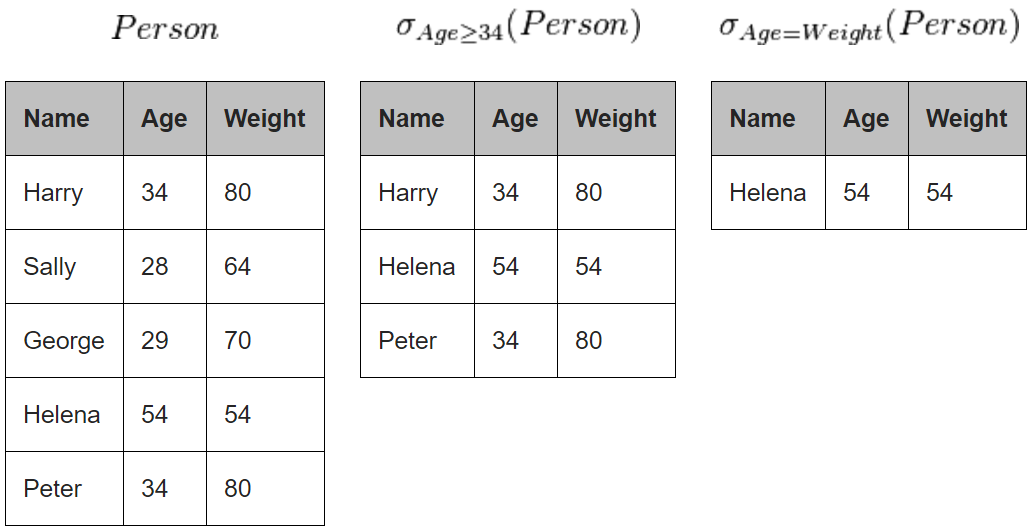
\includegraphics[width=0.8\linewidth]{figs/spm6/select}
	\caption{RA og select.}
	\label{fig:select}
\end{figure}

%Nu kan vi så bruge et \textbf{\textit{select}} statement til at finde alle studerende som har alder over 23, og gennemsnit over 8.
%
%Med relationel algebra vil dette se således ud:
%
%\begin{equation*}
%\sigma_{alder \geq 23}\text{ and } _{gennemsnit \geq 8} (\text{Studerende})
%\end{equation*}
%
%Dette vil så returnere følgende tabel:
%
%\begin{table}[H]
%	\centering
%	\begin{tabular}{lrrl}
%		\toprule
%		\textbf{Navn}	&\textbf{Alder}&\textbf{Gennemsnit}&\textbf{Email}\\
%		\midrule			
%		Hans Hansen		& 45 & 9,8	& hans@landmand.dk	\\			
%		Signe Andersen	& 25 & 8,6	& signe@hotmail.com	\\
%		\bottomrule
%	\end{tabular}
%	\caption{Studerende ældre end 23 med snit over 8.}
%\end{table}
%
%
%På denne måde laver \textbf{\textit{select}} operatoren en \textit{horizontal partition} med to dele: én der opfylder betingelserne og én som ikke gør.
\subsubsection{Project $\pi$}

\url{https://en.wikipedia.org/wiki/Projection_(relational_algebra)}\\

\begin{figure}[h]
	\centering
	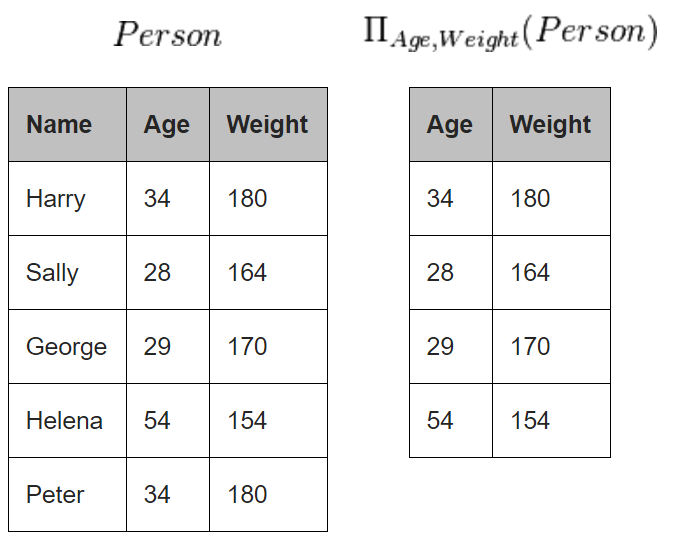
\includegraphics[width=0.6\linewidth]{figs/spm6/project}
	\caption{RA og project}
	\label{fig:project}
\end{figure}


Denne operator bruges til at lave en \textit{vertical partitionering} og giver os kun de kolonner som vi er interesserede i. 
%Eksempelvis, hvis vi kun er interessede i navn og email for alle i tabellen på side~\pageref{tab:stud}, kan vi skrive følgende med RA:
%
%\begin{equation}
%\pi_{navn, email}(Studerende)
%\end{equation}
%
%Hvilket så vil give os følgende tabel:
%
%\begin{table}[H]
%	\centering
%	\begin{tabular}{ll}
%		\toprule
%		\textbf{Navn}	& \textbf{Email}	\\
%		\midrule
%		John Derp		& john@derp.me		\\			
%		Hans Hansen		& hans@landmand.dk	\\			
%		Brian Jensen	& brian@randers.dk	\\			
%		Signe Andersen	& signe@hotmail.com	\\
%		\bottomrule
%	\end{tabular}
%	\caption{Studerende med navn og email.}
%\end{table}
\subsection{Kombination af Project og Select}

Disse operatorer kan også anvendes samtidigt og bruges her til at finde navn og email for studerende, som har et gennemsnit over 7 i tabel~\ref{tab:stud}.

\begin{equation*}
\pi_{navn, email}\sigma_{gennemsnit>7}(Studerende)
\end{equation*}

\begin{lstlisting}[morekeywords={SELECT, FROM, WHERE}]
// SVARE TIL:
SELECT attribute FROM table WHERE condition;
\end{lstlisting}

\begin{table}[H]
	\centering
	\begin{tabular}{lrrl}
		\toprule
		\textbf{Navn}	&\textbf{Alder}	&\textbf{Gennemsnit}&\textbf{Email}\\
		\midrule
		John Derp		& 24 			& 8	& john@derp.me			\\			
		Hans Hansen		& 45 			& 9	& hans@landmand.dk		\\			
		Brian Jensen	& 22 			& 4	& brian@randers.dk		\\			
		Signe Andersen	& 25 			& 10	& signe@hotmail.com		\\
		\bottomrule
	\end{tabular}
	\caption{Tabel: Studerende.}
	\label{tab:stud}
\end{table}

Dette ville så give os følgende tabel:

\begin{table}[H]
	\centering
	\begin{tabular}{ll}
		\toprule
		\textbf{Navn}	& \textbf{Email}	\\
		\midrule
		John Derp		& john@derp.me		\\			
		Hans Hansen		& hans@landmand.dk	\\			
		Signe Andersen	& signe@hotmail.com	\\
		\bottomrule
	\end{tabular}
	\caption{Studerende med snit over 7, kun navn og email.}
\end{table}
\subsubsection{Cartesian Product}

Binær operator. Også kaldet \textit{Cross Product} eller \textit{Cross Join}. 

Kombinere tupler i en relation med alle tupler i en anden relation.

\begin{figure}[h]
\centering
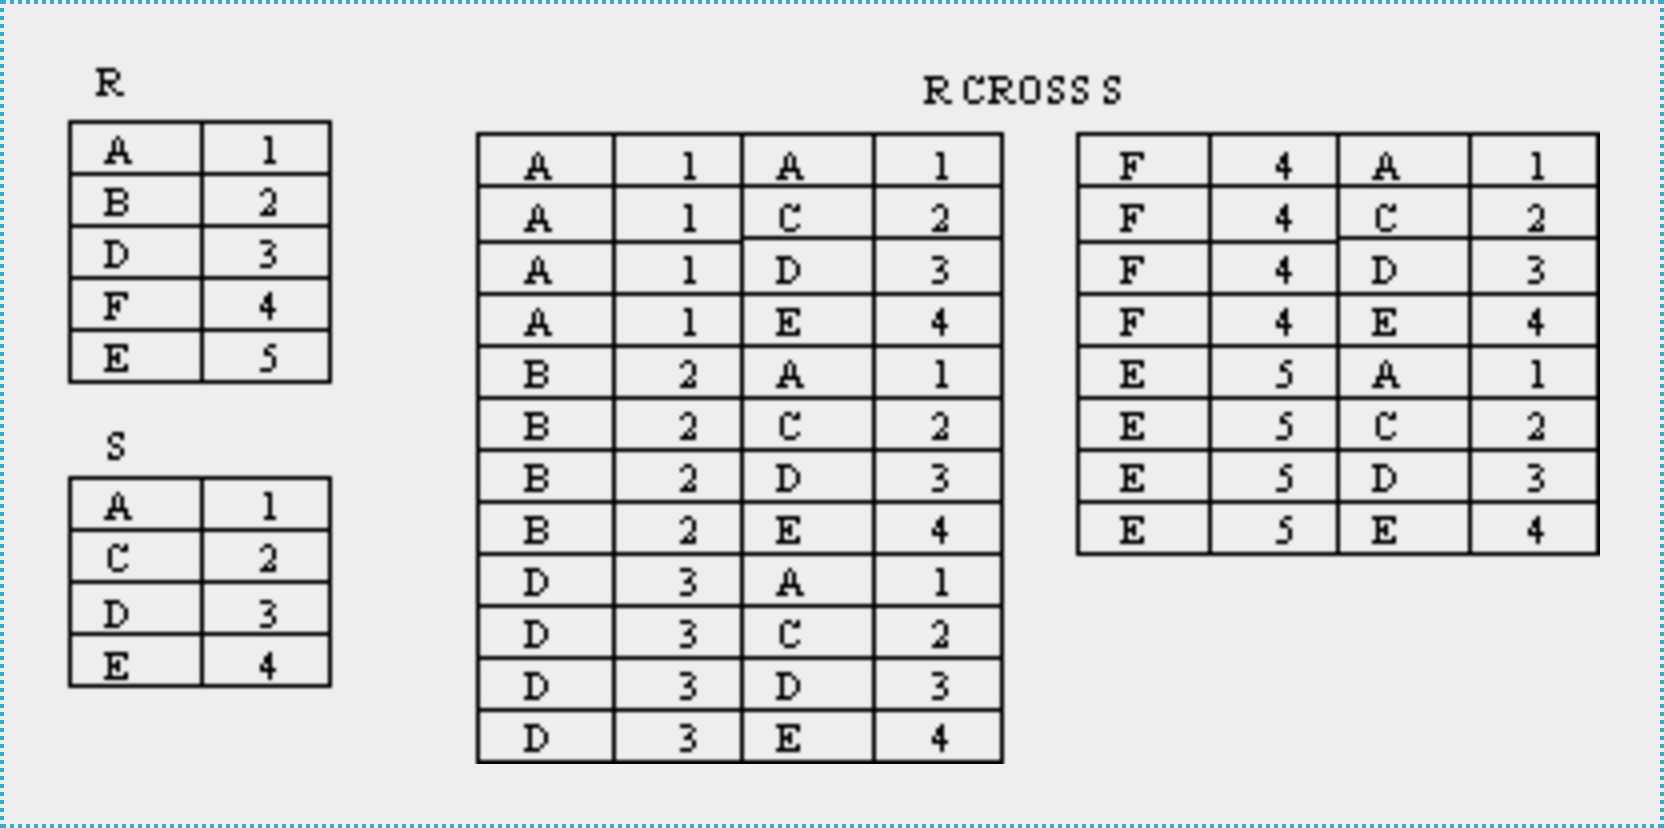
\includegraphics[width=0.8\linewidth]{figs/spm6/cartesianproduct}
\caption{Eksempel på \textit{cartesian product}.}
\label{fig:cartesian_product}
\end{figure}

Som det også kan ses i figur~\ref{fig:cartesian_product} så får hver attribut/kolonne i relation R sin \textit{egen udgave} af hver attribut/kolonne i relation S.

% must
\subsubsection{Samt RA' betydningen for opbygningen af  SQL (Structured Querry Language) erklæringer}



















